\chapter{Introducción}

\section{Motivación para usar MLOps}

Hoy en día, en los proyectos de Machine Learning, el código dedicado a definir los modelos predictivos representa una fracción muy pequeña comparada con otros componentes del flujo de trabajo. Para poder operar con modelos, los científicos de datos deben de trabajar junto con otras personas que se dedican a eso mismo, operaciones (encargados de desplegar, testear el sistema, aprovisionar la infraestructura necesaria, etc). Esto representa un desafío en la organización en términos de comunicación, colaboración y coordinación. El objetivo de MLOps es enfrentarse a dicho desafío estableciendo buenas prácticas para el desarrollo. Además, nos aporta de la velocidad y agilidad necesaria en el mundo digital actual.

\begin{figure}[h]
	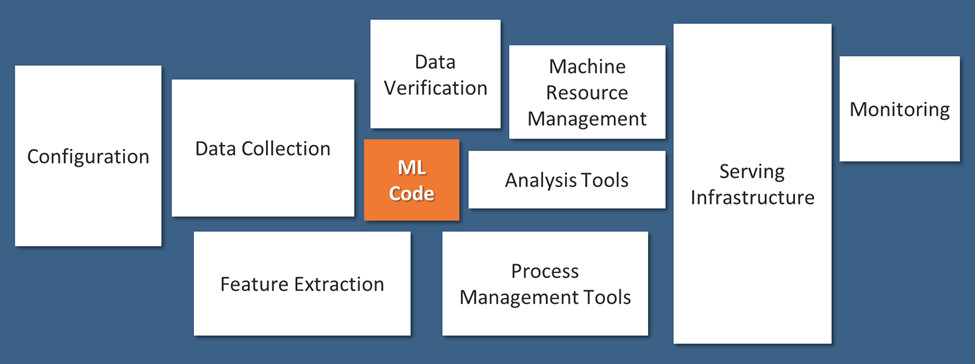
\includegraphics[scale=1]{imagenes/01_Introduccion/mlcodefraction.jpg}
	\centering
	\caption{Como se muestra en la figura, la fracción de código en los sistemas de ML reales es bastante pequeña. En cambio la fracción de infraestructura es mucho mayor \cite{NIPS2015_86df7dcf}.}
\end{figure}

En este caso, adoptar las mejores prácticas de \textbf{DevOps} (una metodología para desarrollo de software basada en la integración entre desarrolladores de software y administradores de sistemas) podría ser posible, pues el Machine Learning tiene mucho en común con la ingeniería del software. La diferencia es que en Machine Learning hay que llevar un registro de modelos y sus hiperparámetros, con el fin de que el experimento se pueda replicar con la mayor facilidad en otro sistema (esto recibe el nombre de reproducibilidad).\newline

En DevOps y MLOps se debe de usar un sistema de control de versiones (git) para poder gestionar los cambios en el código. Adicionalmente, en MLOps necesitamos versionar los modelos y sus hiperparámetros, pero gracias a la herramienta DVC (su uso está explicado en un capítulo posterior) esto ya no es problema. Además de todo lo anterior, el código debe de estar subido a un repositorio remoto compartido (como puede ser GitHub, GitLab, Bitbucket, etc) para poder trabajar cómodamente en equipo. En este repositorio debemos tener el control de que en cada cambio incremental todo lo anterior y lo nuevo siga funcionando, por lo tanto es necesario el uso de lo que se llama Integración Continua. Este proceso de Integración Continua lo que hace es ejecutar los tests que hemos escrito sobre el código implementado para comprobar que efectivamente funciona como esperábamos. En cuanto a MLOps, también es necesario testear que los modelos se comporten como esperamos. Esto nos permite desarrollar software de mayor calidad y con una altísima frecuencia de releases.\newline

Además de lo anterior, también se puede configurar un Despliegue Continuo, así si nuestro código pasa con éxito los tests de Integración Continua, podriamos desplegarlo en cuestión de segundos o unos pocos minutos mediante otras herramientas/plataformas que nos permitan acelerar dicho despliegue usando Infraestructura como Código. Para poder integrar la Integración Continua y el Despliegue Continuo (a partir de ahora lo llamaremos CI/CD) nos hace falta una plataforma en la nube que nos lo permita. Todo esto está desarrollado en los próximos capítulos de este documento.

\section{Descripción del problema}

La Tierra está siendo continuamente \enquote{bombardeada} constantemente con rayos cósmicos que provienen, como su nombre indica, del universo. Estos rayos se componen de partículas que viajan a la velocidad de la luz, que al entrar en contacto con la atmósfera producen una cascada atmosférica extensa. Dicha cascada emite una luz debido a la radiación gamma llamada \enquote{Luz de Cherenkov}. A la misma vez, el rayo cósmico se fragmenta formando hadrones. Es decir, estos rayos se descomponen en una componente hadrónica y otra componente electromagnética.\newline

\enquote{La detección de de rayos gamma de muy alta energía es esencial para investigar las fuentes de la radiación entrante producida por alguno de los fenómenos más extremos que suceden en el universo, por ejemplo estrellas de neutrones y agujeros negros supermasivos} \cite{gonzalez2021tackling}.

\begin{figure}[H]
	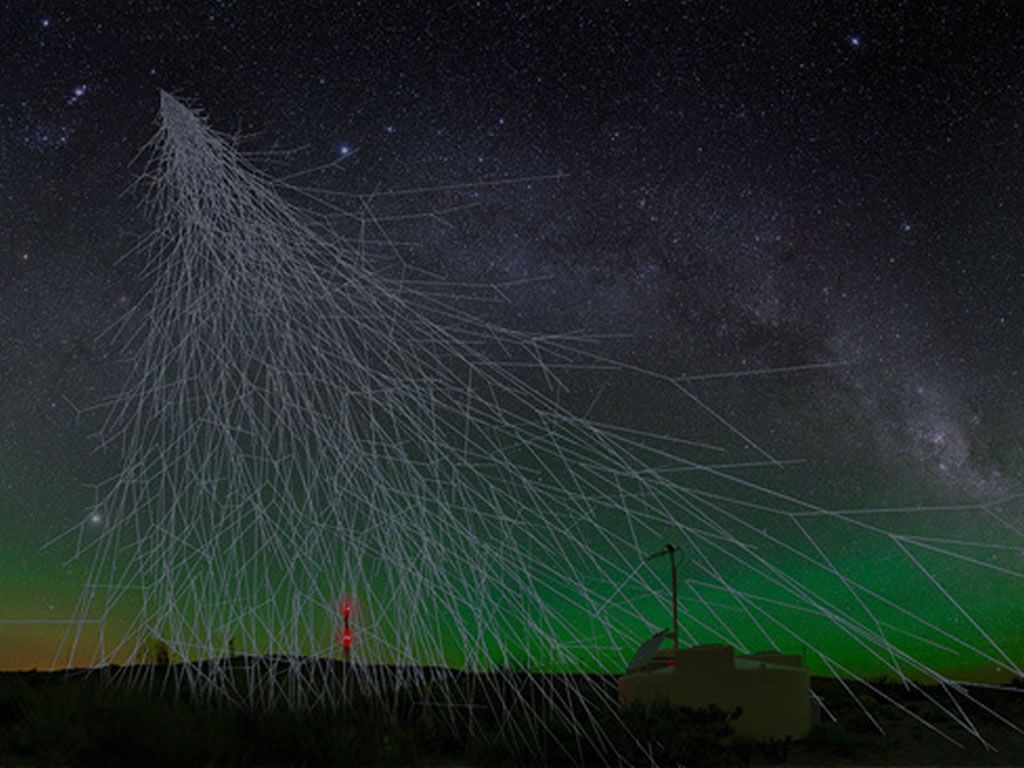
\includegraphics[scale=.3]{imagenes/01_Introduccion/EAS.jpg}
	\centering
	\label{fig:wcd}
	\caption{Así sería una Cascada Atmosférica Extensa incidiendo sobre un Water Cherenkov Detector (WCD). Fuente: \href{https://revolucion.news/cienciario.mx/los-rayos-cosmicos-de-muy-alta-energia-vienen-de-fuera-de-la-via-lactea/}{revolucion.news}.}
\end{figure}

Para poder capturar información sobre dichos rayos cósmicos, se usan WCD (se puede ver la imagen de uno en la Figura \ref{fig:wcd}) que son tanques de agua ultrapura que contienen fotomultiplicadores distribuidos simétricamente dentro del tanque que se utilizan para captar la señal del rayo que incide sobre el tanque. En función de la profundidad del agua del WCD, se emitirá más luz o menos, siendo directamente proporcionales.\newline

El problema que se pretende solucionar en este proyecto, es diseñar un modelo que sea capaz de diferenciar un rayo que sea solo radiación gamma electromagnética de uno que tenga una partícula denominada \enquote{muón}. Esta partícula se genera por la interacción a alta energía de los hadrones y nos permiten discriminar bastante bien entre la radiación gamma y los hadrones \cite{gonzalez2021tackling}.

\begin{figure}[H]
	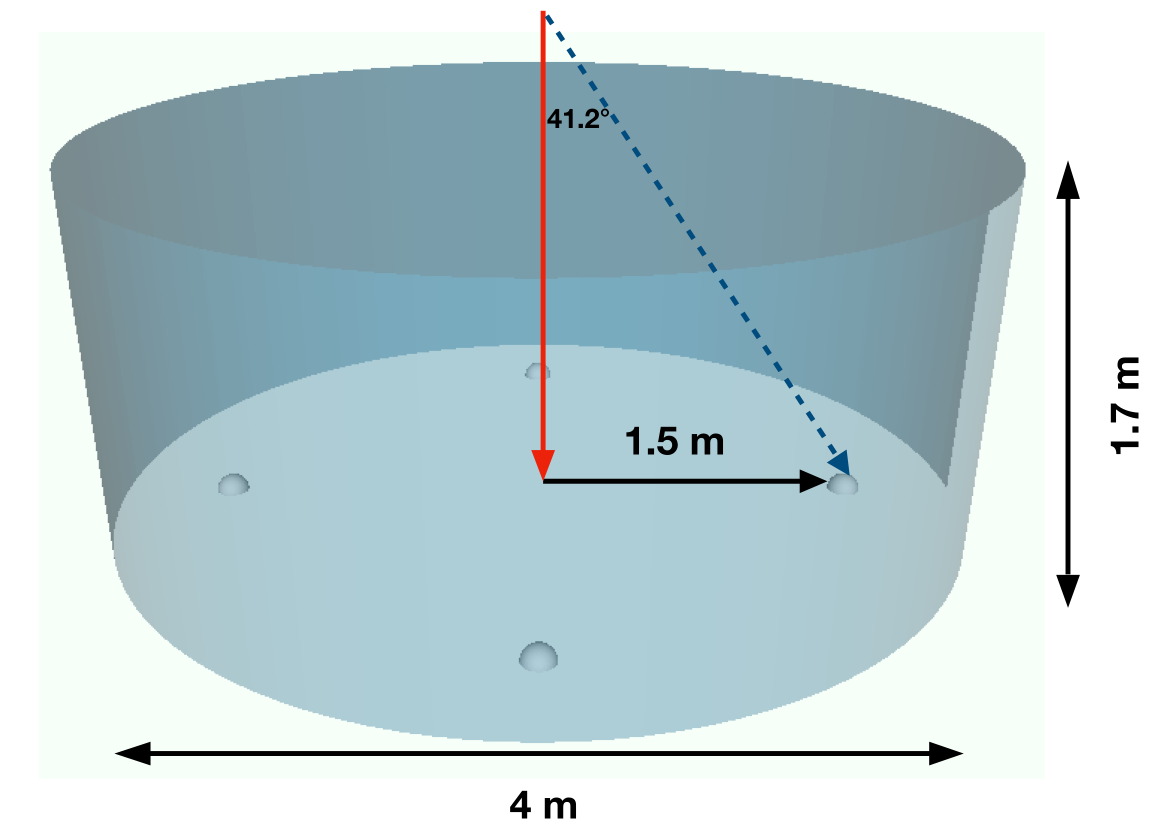
\includegraphics[scale=.1]{imagenes/01_Introduccion/wcd.png}
	\centering
	\caption{Diseño de un WCD \cite{gonzalez2021tackling}.}
\end{figure}
